\chapter{Question5}
\section{问题概述}
%
%%对问题的直观描述
%
本问题要处理的场景中可能有多个幽灵,但是它们的行动是完全随机的,要求为该场景中的基于期望的智能体设计一个评估函数。最终目标是确保吃豆人能够获胜
的前提下,使得分数最大化。

%
%对项目已有代码的阅读和理解
%

%
%解决问题的思路和想法
%

\section{算法设计}
%
%用自己的语言描述解决问题所使用的算法的原理及功能,设计思路和算法流程图
%
本题与第一题的区别在于,这里的评估函数只以给定的状态为参数,而在第一题中,既有状态,也有动作,相当于给出了动作先后的两个状态。这一区别导致的最大的影响在于
我们很难使用某个值的变化量作为评估函数的组成部分。例如,我们无法直接量化时间的流逝,我们只能通过当前的游戏得分来间接反映时间因素——游戏得分会随着时间逐渐减少。
同时,这还会带来一些不方便之处,例如,如果把吃豆人到最近的能量点的距离的倒数作为激励项,来激励吃豆人获取能量点的话,反而会适得其反,因为当吃豆人来到某一能量点
相邻的位置时,此时,如果它吃掉了能量点,那么在这一状态下,到最近的能量点的距离反而增加了,因为最近的能量点更新为了之前的第二近的能量点。这可能会导致吃豆人尽管会被
能量点吸引,但始终不去收集它。

因此,评估函数中的激励项应该满足“递增”的特性,惩罚项要满足“递减”的特性。最终,经过实验,我将评估函数设计为三部分:1)游戏得分;2)到最近的食物的距离的倒数;3)能量点的相反数。
其中,第3项会使得当吃豆人路过能量点时顺带去收集它;第2项中,虽然采用了“最近距离的倒数”的形式,但是并不会导致吃豆人不收集食物的情况,这是因为
食物和能量点不同,收集食物时游戏得分便会增加10分,“最近距离的倒数”最多只会减少1分,因此对于吃豆人而言,收集相邻的食物总是有益的,而
对于能量点,由于收集它时并无法立即得到加分,“最近距离的倒数”反而会减少,如果吃豆人不够“有远见”,即无法搜索博弈树中足够多的层数的话,
它会认为该行为是没有收益的;第一项游戏得分十分重要,因为这一项便能驱使吃豆人在普通状态下远离幽灵,同时主动追逐附近的处于虚弱状态的幽灵。
\section{算法实现}
%
%在算法原理的基础上,结合代码,讲述算法的实现细节、核心函数、模块输入输出,数据结构定义等内容
%
\begin{lstlisting}[emph={[3]currentGameState,gameState,depth,alpha,beta,ghostNo,ghostNum},emphstyle={[3]\color{vscode_parametercolor}},emph={[4]GameState,MinimaxAgent,AlphaBetaAgent},emphstyle={[4]\color{vscode_classcolor}}]
def betterEvaluationFunction(currentGameState: GameState):
    newPos = currentGameState.getPacmanPosition()
    newFood = currentGameState.getFood()
    foods = newFood.asList()
    capsules = currentGameState.getCapsules()
    closeToFood = 0 if not foods else 1 / (min([manhattanDistance(newPos, food) for food in foods]))
    return currentGameState.getScore() + closeToFood - len(capsules)
\end{lstlisting}
\section{实验结果}
%
%对试验结果进行详细展示,对每个问题展示测试截图,对于测试用例进行描述说明,对于为通过测试的用例结合自己的算法进行分析,可以结合调试过程进行分析
%
我成功获得了本问题的所有分数。
\begin{figure}[htbp]
    \centering
    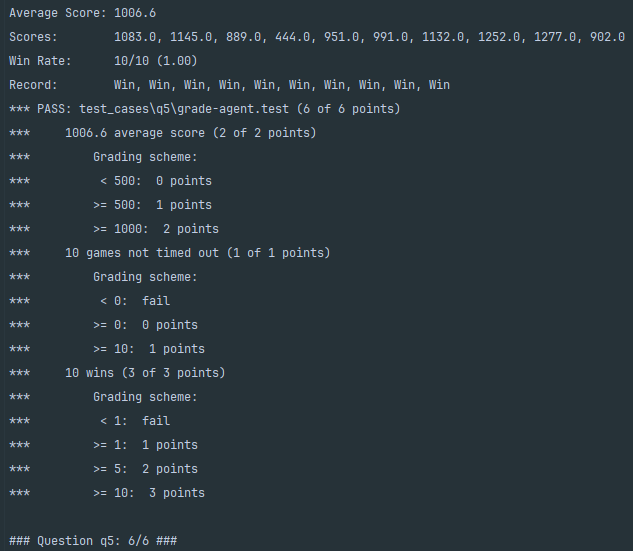
\includegraphics[scale = 0.7]{pic/q6.png}
    \caption{Question6实验结果}\label{q6}
\end{figure}

本问题的测试方式如图\ref{q6test}所示。该测试样例从三个角度评价评估函数的质量:1)得分高低;2)在规定时间内结束游戏;3)获胜率。如果想要获得所有分数,
则吃豆人必须多次吃掉处于虚弱状态下的幽灵。
\begin{figure}[H]
    \centering
    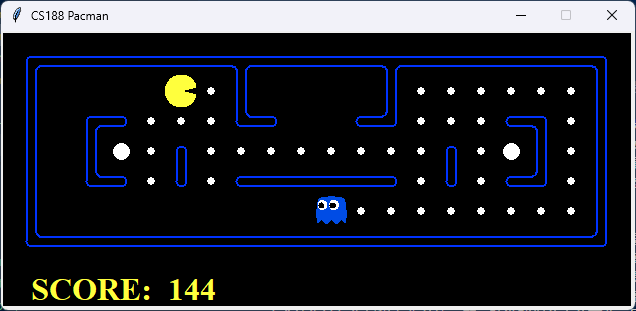
\includegraphics[scale = 0.7]{pic/q6test.png}
    \caption{Question6测试样例}\label{q6test}
\end{figure}
%
%实验中遇到的问题及解决方案,收获和思考:对算法的理解、优缺点的评价、算法的适用场景
%
